\subsection{When Incompleteness Meets Information: Vitali Sets, Signals, and the Limits of Sampling}

\subsubsection{How This Changed Integration Forever}

This wasn’t just a problem for set theorists arguing in dimly lit offices. It had real consequences for how we define \textbf{measure and integration}. Thanks to Gödel, we now know that the sets we assign measure to—the ones we integrate over—are not uniquely determined by logic.

Instead, we have \textbf{choices}. Different models of mathematics allow for different sets to be measurable, and all of them are “correct” within their chosen framework. The question of \textbf{which infinities we allow to have size} is no longer a matter of proof—it’s a matter of preference.

Cantor may have broken mathematics, but Gödel made sure the pieces would never fit back together. 

\subsubsection{When Incompleteness Meets Information: Vitali Sets}

To understand how Gödel’s incompleteness theorem and the Continuum Hypothesis affect modern information theory, we need to revisit one of the strangest objects in mathematics: the \textbf{Vitali set}.

In 1905, the Italian mathematician \textbf{Giuseppe Vitali} used the Axiom of Choice to prove that there exists a subset of the real numbers that is \emph{not} Lebesgue measurable. His construction went like this:

\begin{itemize}
  \item Consider the interval \([0,1]\), and define an equivalence relation where two numbers \( x \sim y \) if \( x - y \) is rational.
  \item This partitions \([0,1]\) into uncountably many disjoint equivalence classes.
  \item Using the Axiom of Choice, select exactly one representative from each class. The resulting set is called a \textbf{Vitali set}.
\end{itemize}

\begin{figure}[H]
\centering
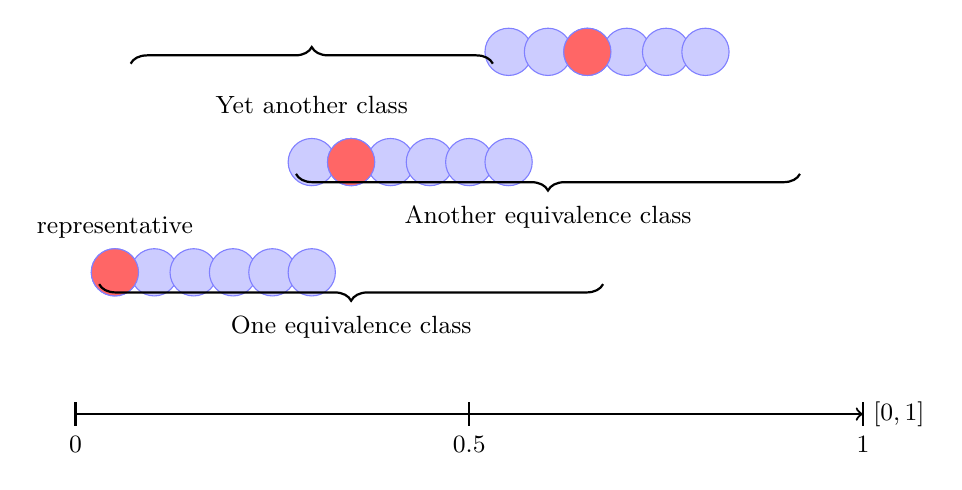
\begin{tikzpicture}[
  every node/.style={font=\small},
  class/.style={circle, fill=blue!20, draw=blue!50, minimum size=0.6cm, inner sep=0pt},
  rep/.style={class, fill=red!60},
  axis/.style={thick, ->},
  tick/.style={thick}
]

% Draw the interval [0,1]
\draw[axis] (0,0) -- (10,0) node[right] {\( [0,1] \)};
\foreach \x/\label in {0/0, 5/0.5, 10/1}
  \draw[tick] (\x,0.15) -- (\x,-0.15) node[below] {\(\label\)};

% Partition dots (rational offsets) — added vertical spacing
\foreach \i/\x in {1/0.5, 2/1.0, 3/1.5, 4/2.0, 5/2.5, 6/3.0}
{
  \node[class] (c\i1) at (\x, 1.8) {};
  \node[class] (c\i2) at ({mod(\x+2.5,10)}, 3.2) {};
  \node[class] (c\i3) at ({mod(\x+5.0,10)}, 4.6) {};
}

% Representatives
\node[rep, label=above:{representative}] at (0.5,1.8) {};
\node[rep] at (3.5,3.2) {};
\node[rep] at (6.5,4.6) {};

% Braces and labels for classes — spaced vertically
\draw[decorate,decoration={brace,mirror,amplitude=6pt}, thick] (0.3,1.65) -- (6.7,1.65) node[midway, below=8pt] {One equivalence class};
\draw[decorate,decoration={brace,mirror,amplitude=6pt}, thick] (2.8,3.05) -- (9.2,3.05) node[midway, below=8pt] {Another equivalence class};
\draw[decorate,decoration={brace,mirror,amplitude=6pt}, thick] (5.3,4.45) -- (0.7,4.45) node[midway, below=8pt] {Yet another class};

\end{tikzpicture}
\caption{Constructing the Vitali set: choose one point from each rational-shifted equivalence class within \([0,1]\). This set defies Lebesgue measure.}
\end{figure}

\medskip

To understand how strange this is, think about how we normally measure subsets of the real line. If you shift a set to the left or right, its length stays the same—this is called translation invariance. If you break a set into countably many disjoint parts and measure each one, their lengths should add up: this is countable additivity. 

\begin{quote}
If a set is well-behaved in a certain technical sense (i.e., Borel or Lebesgue measurable), then we say it’s complete with respect to the measure. And, the Vitali set breaks all of these intuitions.
\end{quote}

It’s not that we don’t know how to measure it. It’s that we provably can’t—not without violating at least one of the axioms that make Lebesgue measure work. If you try to assign it a length, you’ll quickly run into contradictions: either you lose translation invariance, or you give up countable additivity, or your measure becomes incomplete.

\begin{figure}[H]
\centering
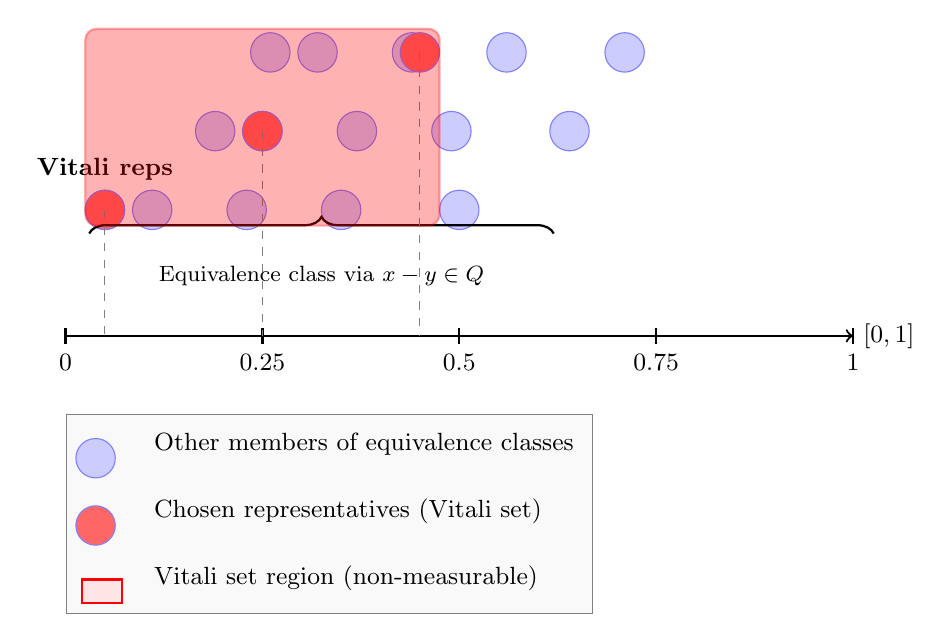
\begin{tikzpicture}[
  every node/.style={font=\small},
  class/.style={circle, fill=blue!20, draw=blue!50, minimum size=0.5cm, inner sep=0pt},
  rep/.style={class, fill=red!60},
  axis/.style={thick, ->},
  tick/.style={thick}
]

% Draw the interval [0,1]
\draw[axis] (0,0) -- (10,0) node[right] {\( [0,1] \)};
\foreach \x/\label in {0/0, 2.5/0.25, 5/0.5, 7.5/0.75, 10/1}
  \draw[tick] (\x,0.1) -- (\x,-0.1) node[below] {\(\label\)};

% Rational translations (classes)
\foreach \i/\x in {1/0.5, 2/1.1, 3/2.3, 4/3.5, 5/5.0}
{
  \node[class] (c\i1) at ({mod(\x,10)}, 1.6) {};
  \node[class] (c\i2) at ({mod(\x+1.4,10)}, 2.6) {};
  \node[class] (c\i3) at ({mod(\x+2.1,10)}, 3.6) {};
}

% Representatives
\node[rep, label=above:{\textbf{Vitali reps}}] at (0.5,1.6) {};
\node[rep] at (2.5,2.6) {};
\node[rep] at (4.5,3.6) {};

% Braces and annotations
\draw[decorate,decoration={brace,amplitude=6pt}, thick] (0.3,1.3) -- (6.2,1.3) node[midway, below=8pt] {\footnotesize Equivalence class via \(x - y \in \mathbb{Q}\)};
\draw[dashed, gray] (0.5,1.6) -- (0.5,0);
\draw[dashed, gray] (2.5,2.6) -- (2.5,0);
\draw[dashed, gray] (4.5,3.6) -- (4.5,0);

% Vitali set region (implicit)
\draw[fill=red!10, rounded corners, thick, red, opacity=0.3] (0.25,1.4) rectangle (4.75,3.9);

% LEGEND (scaled down)
\begin{scope}[scale=0.66, shift={(0,-1.5)}]
\matrix[draw=black!50, fill=gray!5, column sep=8pt, row sep=4pt, anchor=north west] {
  \node[class] {}; & \node[anchor=west]{Other members of equivalence classes}; \\
  \node[rep] {};   & \node[anchor=west]{Chosen representatives (Vitali set)}; \\
  \node[fill=red!10, minimum width=0.5cm, minimum height=0.3cm, draw=red, thick] {}; & \node[anchor=west]{Vitali set region (non-measurable)}; \\
};
\end{scope}

\end{tikzpicture}
\caption{The Vitali set: by selecting one representative from each rational-translation equivalence class in \([0,1]\), we construct a set that is fundamentally non-measurable. The legend shows how the construction is visualized.}
\end{figure}

In other words: the Vitali set is a kind of mathematical ghost. It “exists” (if you accept the Axiom of Choice), but it refuses to behave. It lurks outside the bounds of what our mathematical tools can grasp cleanly—just like Gödel’s incompleteness theorem shows that some truths exist outside the bounds of what formal systems can prove.





